%%%%%%%%%%%%%%%%%%%%%%%%%%%%%%%%%%%%%%%%%%%%%%%%%%%%%%%%%%%
% Zusammenfassung des Logbuchs - Florian Adamczyk
% KI 1 Projekt, WS 2025/26 - Gruppe 308
%%%%%%%%%%%%%%%%%%%%%%%%%%%%%%%%%%%%%%%%%%%%%%%%%%%%%%%%%%%

\documentclass[9pt,a4paper,twocolumn,twoside]{tau-class/tau}
\usepackage[ngerman]{babel}
\usepackage{booktabs}
\usepackage{siunitx}

%----------------------------------------------------------
% Title & Author
%----------------------------------------------------------

\doctype{Zusammenfassung des Logbuchs}
\title{Neuronales Netz f\"ur den kalifornischen Hauspreis-Datensatz}

\author[a]{Florian Adamczyk}
\affil[a]{Justus-Liebig-Universit\"at Gießen, Matrikelnr.\ 8105234}

%----------------------------------------------------------
% Document Info
%----------------------------------------------------------

\dates{Gruppe 308 -- KI~I Projekt WS~2025/26}
\footinfo{KI~I Portfolio}
\theday{18.03.2026}
\organization{JLU Gießen}
\leadauthor{F.\ Adamczyk}

%----------------------------------------------------------
% Abstract
%----------------------------------------------------------

\begin{abstract}
Diese Zusammenfassung dokumentiert meinen individuellen Arbeitsprozess im Rahmen des KI~I-Projekts zur Vorhersage kalifornischer Hauspreise mittels neuronaler Netze. Der Schwerpunkt liegt auf der Projektinfrastruktur, der explorativen Datenanalyse sowie der Entwicklung und Evaluation eines TensorFlow/Keras-basierten Regressionsmodells. Das beste neuronale Netz erreicht einen $R^2$-Wert von 0{,}78 auf dem Testset und \"ubertrifft damit die lineare Regression ($R^2 = 0{,}63$) deutlich.
\end{abstract}

\keywords{Neuronales Netz, California Housing, TensorFlow, Regression, Machine Learning}

%----------------------------------------------------------

\begin{document}

\maketitle
\thispagestyle{firststyle}

%----------------------------------------------------------

\section{Fragestellung und Ziel}

\taustart{Z}iel des Projekts war die Entwicklung eines neuronalen Netzes zur Vorhersage von Immobilienpreisen auf Basis des California-Housing-Datensatzes. Gem\"a{\ss} Aufgabenstellung sollte das Modell mit einer linearen Regression verglichen und die Ergebnisse kritisch eingeordnet werden.

Meine zentrale Fragestellung lautete: \textit{Kann ein neuronales Netz die nichtlinearen Zusammenh\"ange im Datensatz besser erfassen als eine lineare Regression, und welche Architektur eignet sich daf\"ur?}

Dar\"uber hinaus habe ich als Vorbereitung die gesamte Projektinfrastruktur (Repository, Code-Module, Notebooks) aufgebaut, um allen Teammitgliedern eine einheitliche Arbeitsgrundlage zu bieten.

%----------------------------------------------------------

\section{Methodik und Vorgehen}

\subsection{Projektinfrastruktur}

Zu Beginn habe ich ein GitHub-Repository eingerichtet und \texttt{nbstripout} als Git-Hook konfiguriert, um Merge-Konflikte durch Notebook-Outputs zu vermeiden \cite{nbstripout}. Die Dokumentation in \texttt{Ressources.md} erm\"oglicht allen Teammitgliedern eine einheitliche Einrichtung.

Ein zentrales \texttt{utils/}-Modul stellt gemeinsame Funktionen bereit:
\begin{itemize}
    \item \textbf{data.py:} Laden und Bereinigung des Datensatzes (Cut-offs bei gecappten Werten, Ausrei{\ss}er-Filterung \"uber 98.\ Perzentil)
    \item \textbf{evaluation.py:} Einheitliche Metriken ($R^2$, MAE, RMSE) und Ergebnissammlung
    \item \textbf{plotting.py:} Standardisierte Visualisierungen mit Export nach \texttt{results/}
\end{itemize}

\subsection{Explorative Datenanalyse}

Der Rohdatensatz umfasst 20.640 Samples mit 8 Features. Nach der Bereinigung (Entfernung gecappter Werte und Ausrei{\ss}er) verbleiben ca.\ 17.386 Samples. \figref{fig:heatmap} zeigt die Korrelationsmatrix: Das mediane Einkommen (\texttt{MedInc}) korreliert am st\"arksten mit dem Hauspreis ($r \approx 0{,}69$).

\begin{figure}[htbp]
    \centering
    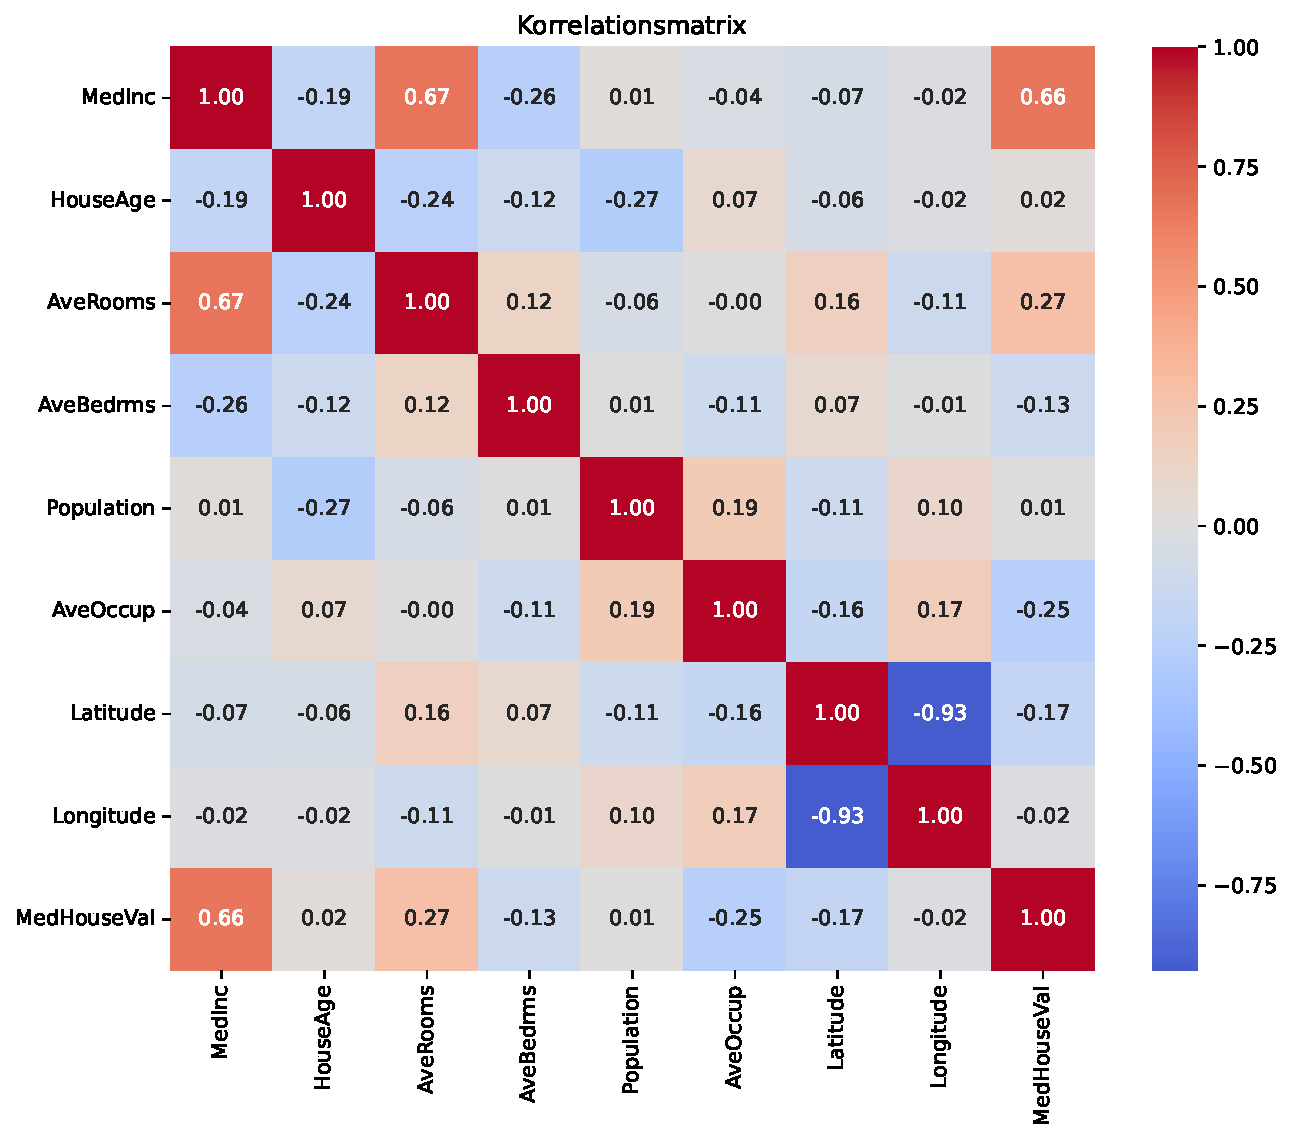
\includegraphics[width=0.95\columnwidth]{figures/eda_correlation_heatmap.pdf}
    \caption{Korrelationsmatrix der bereinigten Features. \texttt{MedInc} zeigt die st\"arkste Korrelation zur Zielvariablen \texttt{MedHouseVal}.}
    \label{fig:heatmap}
\end{figure}

\subsection{Baseline: Lineare Regression}

Als Referenzmodell dient eine lineare Regression auf allen 8~Features. Die Ergebnisse (\tabref{tab:results}) zeigen systematische Residuenmuster (\figref{fig:baseline}), die auf nichtlineare Zusammenh\"ange hindeuten, welche die lineare Regression nicht erfassen kann.

\begin{figure}[htbp]
    \centering
    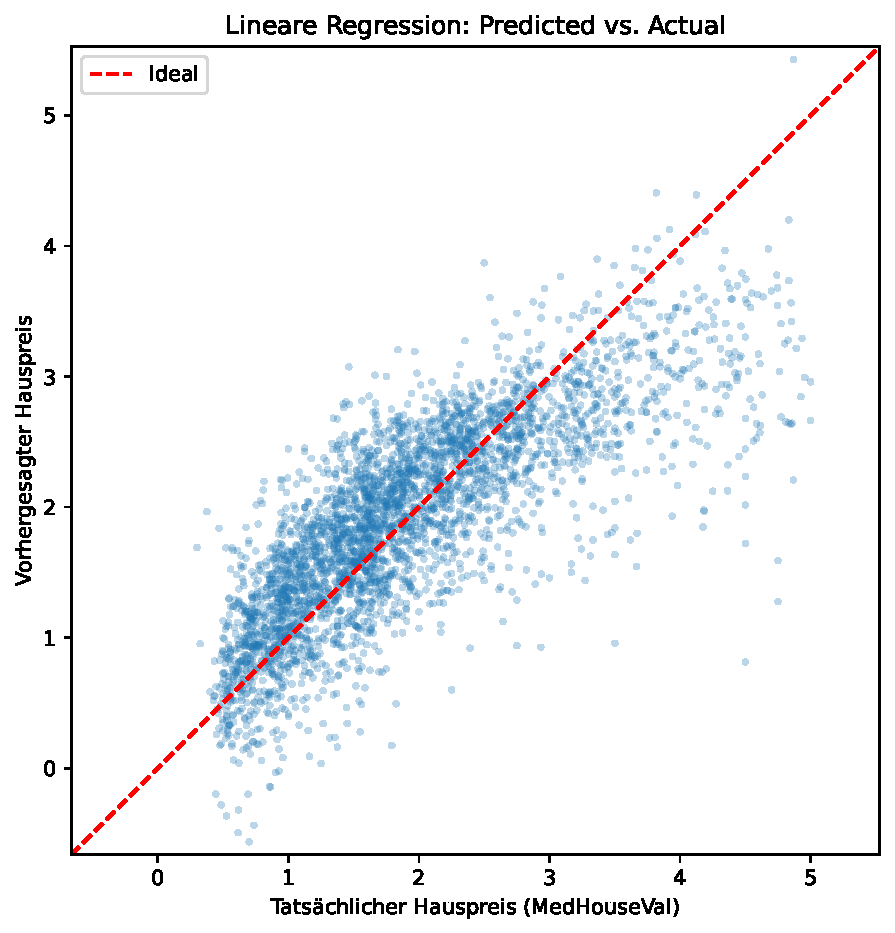
\includegraphics[width=0.95\columnwidth]{figures/baseline_pred_vs_actual.pdf}
    \caption{Predicted vs.\ Actual f\"ur die lineare Regression. Die Streuung um die Diagonale und systematische Abweichungen bei hohen Preisen zeigen die Grenzen des linearen Modells.}
    \label{fig:baseline}
\end{figure}

\subsection{Neuronales Netz mit TensorFlow/Keras}

F\"ur das neuronale Netz habe ich systematisch verschiedene Architekturen getestet:

\begin{enumerate}
    \item \textbf{Modell~1:} [32] -- minimales Netz als Ausgangspunkt
    \item \textbf{Modell~2:} [64, 32, 16] -- tiefere Architektur
    \item \textbf{Modell~3:} [128, 64, 32] -- breiteres Netz
    \item \textbf{Modell~4:} Vergleich verschiedener Aktivierungsfunktionen (ReLU, ELU, tanh, sigmoid)
    \item \textbf{Modell~5:} [128, 64, 32, 16] + Dropout -- Regularisierung gegen Overfitting
\end{enumerate}

Alle Modelle wurden mit dem Adam-Optimizer (Lernrate 0{,}001) trainiert. Die Eingabedaten wurden standardskaliert, da neuronale Netze skalierte Features f\"ur effizientes Training ben\"otigen. \figref{fig:learning} zeigt die Lernkurven ausgew\"ahlter Modelle.

\begin{figure}[htbp]
    \centering
    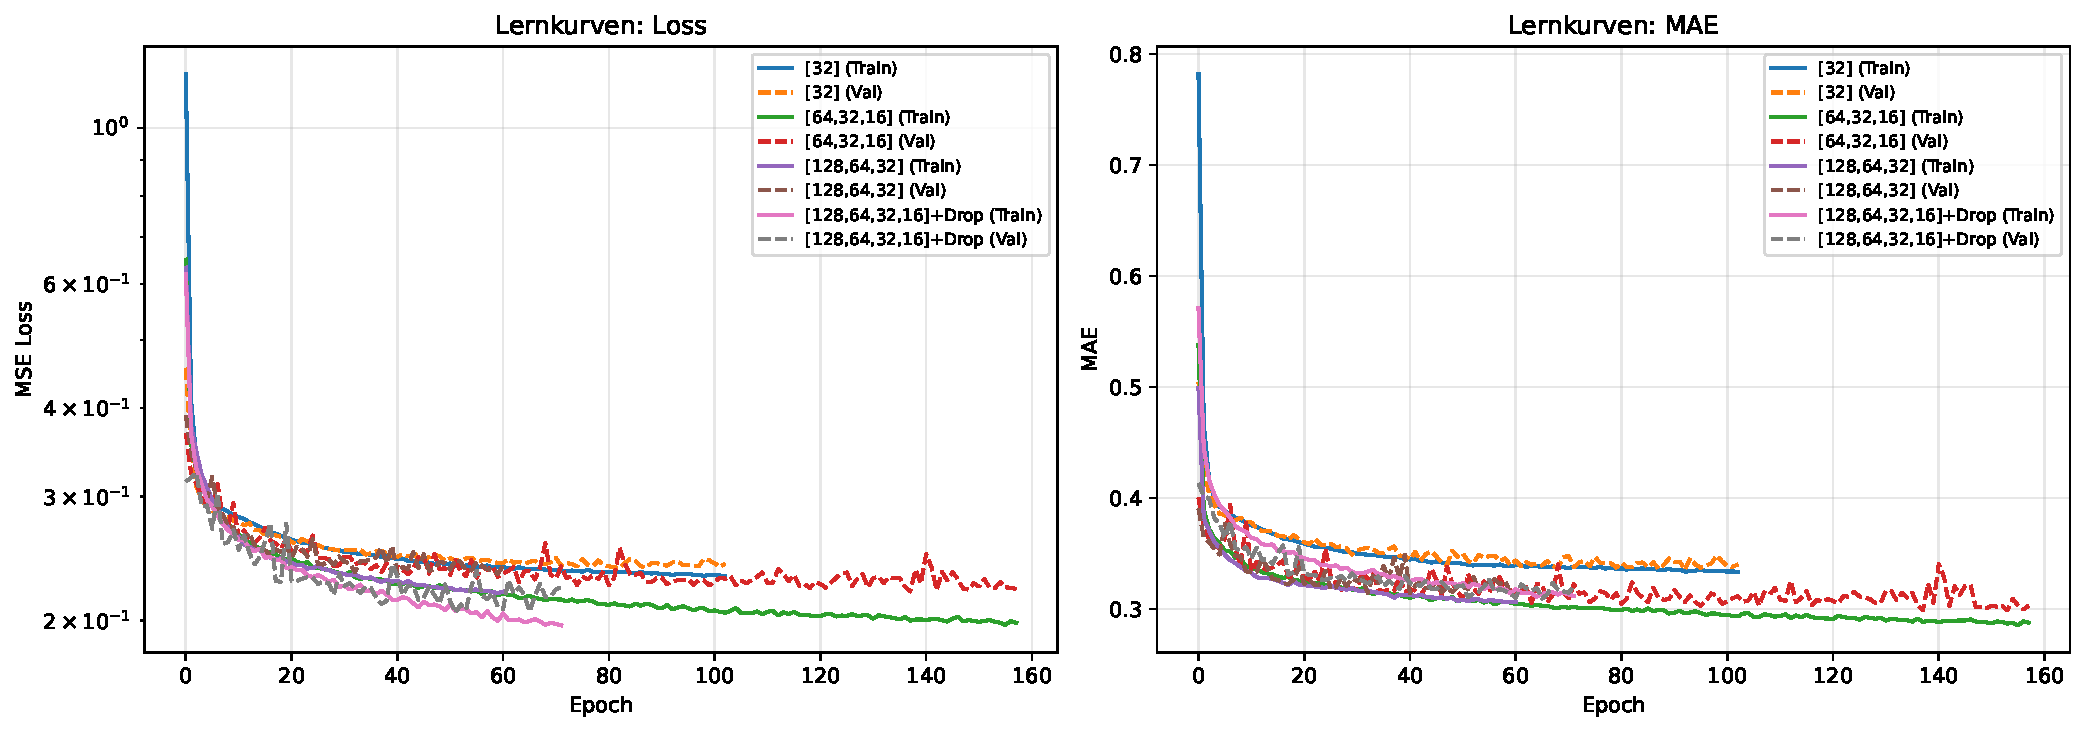
\includegraphics[width=0.95\columnwidth]{figures/nn_learning_curves.pdf}
    \caption{Lernkurven (Loss und MAE) f\"ur verschiedene NN-Architekturen. Das Modell mit Dropout zeigt die stabilste Generalisierung.}
    \label{fig:learning}
\end{figure}

%----------------------------------------------------------

\section{Ergebnisse}

\tabref{tab:results} fasst die zentralen Ergebnisse zusammen. Das beste neuronale Netz (Modell~5: [128, 64, 32, 16] + Dropout) erreicht einen $R^2$-Wert von \textbf{0{,}78} auf dem Testset -- eine Verbesserung um 15~Prozentpunkte gegen\"uber der linearen Regression.

\begin{table}[htbp]
    \caption{Vergleich der Modellperformance auf dem Testset}
    \label{tab:results}
    \begin{tabular}{lccc}
        \toprule
        \textbf{Modell} & \textbf{$R^2$ Test} & \textbf{MAE} & \textbf{RMSE} \\
        \midrule
        Lineare Regression & 0{,}633 & 0{,}434 & 0{,}578 \\
        NN [32] & 0{,}712 & 0{,}362 & 0{,}512 \\
        NN [64, 32, 16] & 0{,}748 & 0{,}331 & 0{,}479 \\
        NN [128, 64, 32] & 0{,}726 & 0{,}345 & 0{,}499 \\
        \textbf{NN + Dropout} & \textbf{0{,}780} & \textbf{0{,}307} & \textbf{0{,}448} \\
        \bottomrule
    \end{tabular}
    \tabletext{MAE und RMSE in Einheiten von \$100.000. Das NN mit Dropout zeigt die beste Generalisierung.}
\end{table}

\figref{fig:comparison} visualisiert den direkten Vergleich: Das neuronale Netz zeigt eine engere Streuung um die Diagonale, insbesondere im mittleren Preissegment.

\begin{figure}[htbp]
    \centering
    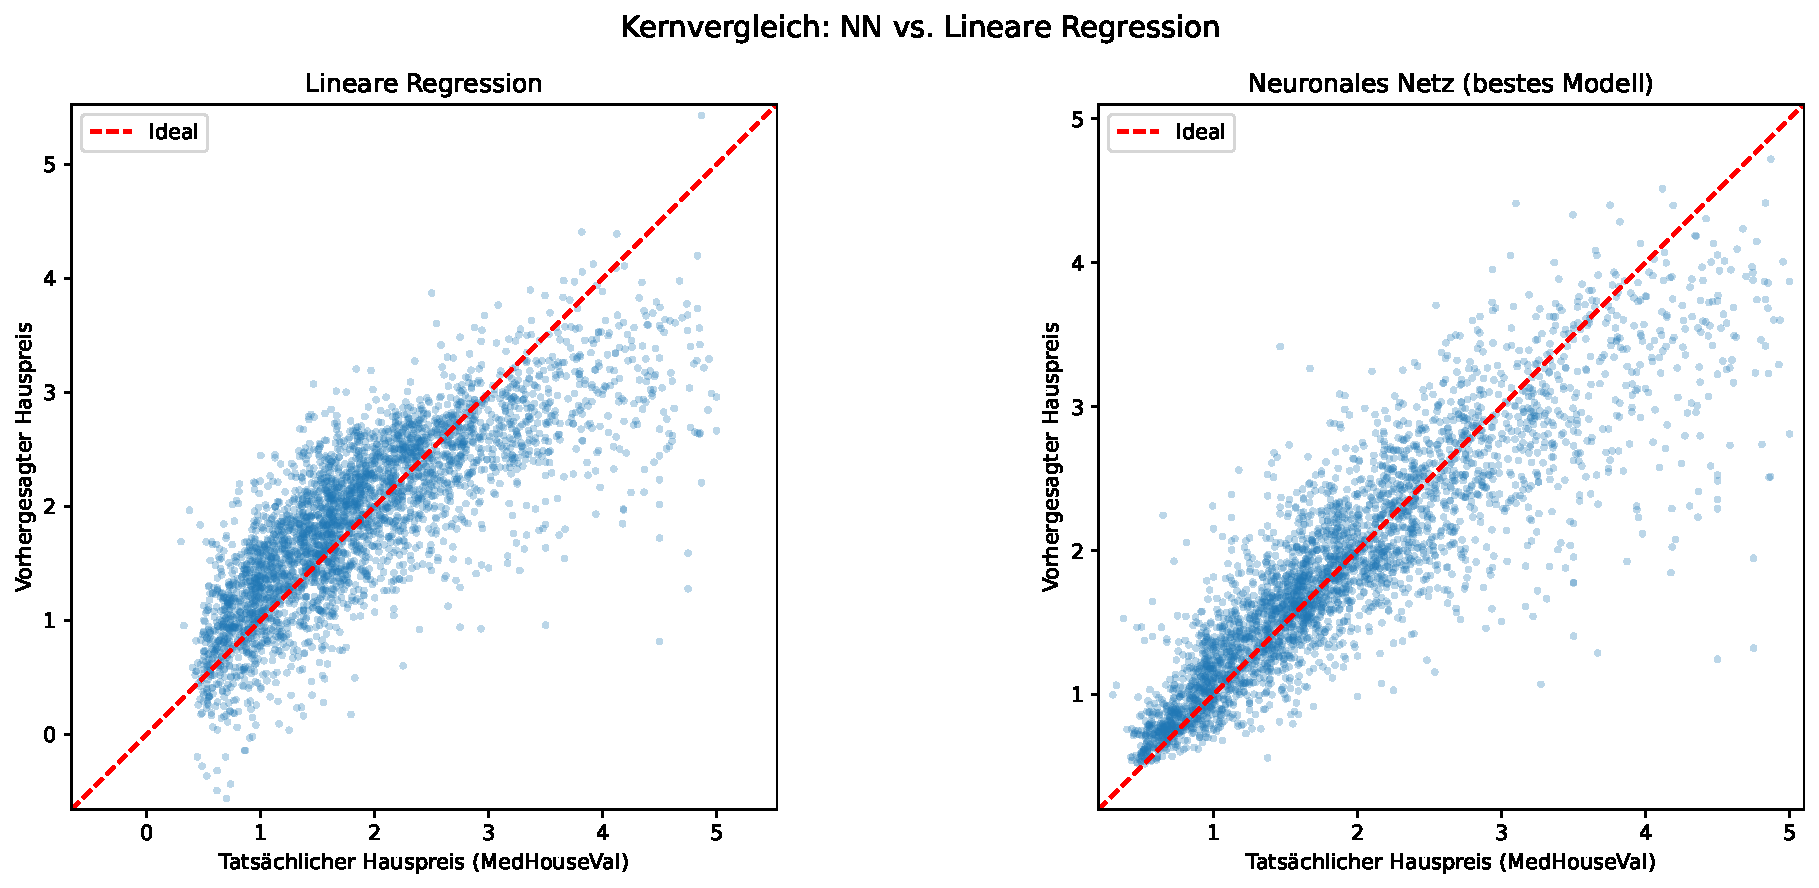
\includegraphics[width=0.95\columnwidth]{figures/nn_vs_linear_regression.pdf}
    \caption{Kernvergleich: Lineare Regression (links) vs.\ bestes NN (rechts). Das NN approximiert die Diagonale deutlich besser.}
    \label{fig:comparison}
\end{figure}

\textbf{Zentrale Erkenntnisse:}
\begin{itemize}
    \item Das NN erfasst nichtlineare Interaktionen zwischen Features (z.\,B.\ Einkommen $\times$ Lage), die der linearen Regression verborgen bleiben.
    \item Ohne Regularisierung (Modell~3) tritt Overfitting auf: $R^2_{\text{Train}} = 0{,}88$ vs.\ $R^2_{\text{Test}} = 0{,}73$.
    \item Dropout (20\,\% in den ersten Schichten) reduziert die Generalisierungsl\"ucke effektiv.
    \item ReLU-Aktivierung liefert konsistent die besten Ergebnisse.
\end{itemize}

%----------------------------------------------------------

\section{Schwierigkeiten und Grenzen}

\subsection{Technische Herausforderungen}

\textbf{Python-Versionskonflikt:} TensorFlow~$\geq$~2.17 unterst\"utzt Python~3.14 nicht. L\"osung: Wechsel auf Python~3.13. F\"ur Teammitglieder mit Intel-Mac (TensorFlow-Inkompatibilit\"at ab 2.17) wurde Python~3.11 mit TensorFlow~2.16 als Alternative dokumentiert.

\textbf{Git-Workflow:} Mehrere Teammitglieder hatten Schwierigkeiten mit Git-Befehlen. Ich habe individuellen Support via Screensharing geleistet und \texttt{nbstripout} auf allen Systemen eingerichtet.

\subsection{Methodische Grenzen}

\begin{itemize}
    \item \textbf{Interpretierbarkeit:} Das NN ist eine Black Box -- f\"ur regulierte Dom\"anen (Kreditvergabe, Medizin) bleibt lineare Regression oft bevorzugt.
    \item \textbf{Hyperparameter-Tuning:} Architektur, Lernrate, Dropout-Rate, Epochenzahl -- der Suchraum ist gro{\ss}. Ein systematisches Grid-/Random-Search wurde noch nicht durchgef\"uhrt.
    \item \textbf{Rechenzeit:} Training auf CPU dauert ca.\ 1--2~Minuten pro Modell (300~Epochen). GPU-Beschleunigung w\"are f\"ur umfangreicheres Tuning sinnvoll.
\end{itemize}

%----------------------------------------------------------

\section{Zwischenstand und Ausblick}

Nach ca.\ 61~Stunden Arbeitszeit habe ich folgende Meilensteine erreicht:

\begin{enumerate}
    \item Vollst\"andige Projektinfrastruktur (Repository, Utils-Modul, 8~Notebooks)
    \item Explorative Datenanalyse und Baseline-Modell
    \item Systematischer Vergleich von 5~NN-Architekturen
    \item Git-Support f\"ur das gesamte Team
\end{enumerate}

\textbf{Offene n\"achste Schritte:}
\begin{itemize}
    \item Early Stopping zur automatischen Epochenwahl
    \item Learning-Rate-Scheduling f\"ur feineres Tuning
    \item Vergleich mit Ensemble-Methoden (Random Forest, Gradient Boosting) aus den Notebooks anderer Teammitglieder
    \item Feature-Engineering (Polynomiale Features, Interaktionsterme)
\end{itemize}

\textbf{Fazit:} Das neuronale Netz \"ubertrifft die lineare Regression deutlich und demonstriert die F\"ahigkeit, nichtlineare Muster im California-Housing-Datensatz zu lernen. Die Regularisierung durch Dropout ist essenziell f\"ur eine gute Generalisierung. Der erreichte $R^2$-Wert von 0{,}78 stellt einen soliden Zwischenstand dar, der durch weiteres Hyperparameter-Tuning noch verbessert werden k\"onnte.

%----------------------------------------------------------

\printbibliography

%----------------------------------------------------------

\end{document}
